\section{PLL}
test
\subsection{Principio di funzionamento}

\Figure{}{}{
    \draw[-latex] (0,0) node[left]{$\phi_{in}$} 
                        -- ++(1,0) coordinate(a);
    \draw [fill=lightgray] (a) ++(0,0.5)rectangle ++(2,-1) 
                            node [pos=.5, align=center]{PLL} ++(0,0.5) coordinate (b);
    \draw[-latex] (b) -- ++(1,0) node[right]{$\phi_{out}$} 
    ;
}

Fà in modo che la frequenza di uscita sia uguale alla frequenza di ingresso e questo funziona quando la differenza di fase tra uscita ed ingresso è costante.

il PLL è un sistema di controllo che genera un sistema di controllo la cui fase di uscita è legata alla fase di ingresso.
La fase di uscita segue la fase di ingresso.
In generale l'obiettivo del PLL è fare in modo che $F_{out}=F_{in}$.
Questo si ottiene quando la fase di uscita è agganciata alla fase ingresso, ovvero quando 
la differenza di fase tra uscita e ingresso è costante.
In altre parole, Se questa differenza di fase varia nel tempo, le frequenze dei due segnali non sono uguali.\\
Noi quindi vogliamo sincronizzare la fase in ingresso con quello di uscita, come conseguenza il PLL può seguire
 la frequenza in ingresso oppure può generare nuove frequenze multiple di quella di ingresso.\\
\\
DISEGNO GRAFICO XOR\\
\\


\Figure{}{}{
    \draw[-latex] (0,0)-- ++(1,0) coordinate(a);
    \draw (a) ++(0,0.25)rectangle ++(2,-1)
        node [pos=.5, align=center]{PD} ++ (0,0.5) coordinate (b);
    \draw[-latex] (b)-- ++(1.5,0) coordinate(c);
    
    \draw (c) ++(0,0.5)rectangle ++(2,-1)
        node [pos=.5, align=center]{VCO} coordinate (d);
    \draw[-latex] (1+2+1.5+1,-0.75) --++(0,-0.75) 
        --++ (-5,0) --++ (0,0.75+0.25) --++ (0.5,0) coordinate (e);

    %draw square wave
    \begin{scope}[scale=0.65]{
        \draw[red] (3+1.9,0)--++(0.25,0)--++(0,+1)--++(0.25,0)--++(0,-1)--++(0.25,0)
        --++(0,+1)--++(0.25,0)--++(0,-1)--++(0.25,0)--++(0,+1)--++(0.25,0)--++(0,-1)--++(0.25,0);
        }
    \end{scope}

    \node[circle,fill=black,inner sep=0pt,minimum size=3pt,label={below:\textcolor{red}{$v_c(t)$}}] (a) at (3.75,-0.25) {};
}
I blocchi principale del PLL sono molto noti ma in questo momento voglio studiare un passo alla volta. 
Nella figura REF si osserva la forma più semplice, sebbene errata perchè incompleta, forma di PLL. 
Da qui si osserva che il PLL sfrutta un feedback negativo. La frequenza di uscita torna in ingresso e la fase di uscita viene comparata con quelal di ingresso, generando
degli impulsi. il VCO quindi riceve gli impulsi e modifica la sua frequenza di uscita secondo una relazione lineare.

\Figure{}{}{
    %disegno asse x
    \draw[-latex,line width=0.75pt](0,0) node[below]{$0$}--(5,0)node[below]{$v_c(t)$};
    %disegno asse y
    \draw[-latex,line width=0.75pt](0,0)--(0,3)node[blue, right]{$f_{out}$};
    %disegno grafico
    \draw[blue] (0,0.5)--(4.5,2.25);
}
Prima di continuare devo ripassare la modulazione FM.
Quello che mi interessa ora, a discapito della correttezza del PLL è lo studio preliminare del VCO.
Se la tensione di controllo del VCO è affetto da ripple succederà che,  insieme alla componente fondamentale si 
genereranno bande laterali. cioè il ripple modula la vco e genera nuovi contributi in frequenza.

REMINDER FM MODULATION\\
Immaginiamo che VCO applichi una modulazione FM e che la sua uscita sia il risultato di una modulazione con un segnale
di ingresso supposto a bassa frequenza (o anche alta).
\Figure{}{}{
    \draw[line width = 1pt](0,0)node[left]{$x_{BB}(t)$} --++(1.5,0)
    % Place a circle labeled VCO at the midpoint of the line
        node[circle, fill=lightgray, minimum size=1.5cm, label=center:{VCO}] {}
            --++ (1.5,0)node[right]{$v_{out}(t)$};
    %disegno perimetro cerchio
    % Draw the outer perimeter circle
        \draw [line width = 0.75pt] (1.5,0) circle[radius=0.75cm];
}
La tensione di uscita si esprime in generale come:
\begin{equation}
    v_{out}=\sin{\left(\omega_c t +K_{vco}\int x_{BB}(t)\right)}
\end{equation}
Dove ho scritto la fase come $Phase=\int Frequency$. Dove la fase phi= è Kvcointxbb(t) e sò che la fase è integrale della frequenza
nel nostro caso, per esempio

\begin{equation}
    v_{out}=\sin{\left( (\omega_c +K_{vco} v_1)\cdot t\ \right)}
\end{equation}
Il termine $\omega_c +K_{vco} v_1$ è la frequenza di uscita $\omega_{out}$ ed è utile notare come essa
sia direttamente proporzionale alla tensione di ingresso $V_1$ secondo una relazione lineare.

\Figure{}{}{
    %disegno asse x
    \draw[-latex,line width=0.75pt](0,0) node[below]{$0$}--(5,0)node[below]{$v_c(t)$};
    %disegno asse y
    \draw[-latex,line width=0.75pt](0,0)--(0,3)node[right]{$f_{out}$};
    %disegno grafico
    \draw[black] (0,0.5)node[left]{$\omega_c$}--(4.5,2.25);

    %disegno label e tratteggi
    \draw[dashed] (0,1.95)node[left]{$\omega_c+K_{vco}\cdot v_1$}--(3.75,1.95);
    \draw[dashed] (3.75,0)node[below]{$v_1$}--(3.75,1.95);
    \node[circle, draw=black, fill=white,inner sep=2.5pt,minimum size=4pt] at (3.75,1.95){};
     
}


\Figure{}{}{
    \draw[-latex] (0,0)-- ++(1,0) coordinate(a);
    %draw PD
    \draw (a) ++(0,0.25)rectangle ++(2,-1)
        node [pos=.5, align=center]{PD} ++ (0,0.5) coordinate (b);
    \draw[-latex] (b)-- ++(1.5,0) coordinate(c);
    %draw LPF
    \draw (c) ++(0,0.5)rectangle ++(2,-1)
        node [pos=.5, align=center]{LPF} ++ (0,0.5) coordinate (d);
    \draw[-latex] (d)-- ++(1.5,0) coordinate(e);
    %draw VCO
    \draw (e) ++(0,0.5)rectangle ++(2,-1)
        node [pos=.5, align=center]{VCO};
    %feedback
    \draw[-latex] (1+2+1.5+2+1.5+1,-0.75) --++(0,-0.75) 
        --++ (-5-1.5-2,0) --++ (0,0.75+0.25) --++ (0.5,0) ;

    %draw square wave
    \begin{scope}[scale=0.65]{
        \draw[red] (3+1.9,0)--++(0.25,0)--++(0,+1)--++(0.25,0)--++(0,-1)--++(0.25,0)
        --++(0,+1)--++(0.25,0)--++(0,-1)--++(0.25,0)--++(0,+1)--++(0.25,0)--++(0,-1)--++(0.25,0);
        }
    \end{scope}

    %draw filter output
    \begin{scope}[scale=0.65]{
        \draw[red] (6.5+3.7,0)--++(0.25,0)--++(0.2,0.4)--++(0.05,-0.4)--++(0.25,0)--++(0.25,0.4)--++((0.05,-0.4)--++(0.25,0)--++(0.25,0.4)--++(0.05,-0.4)--++(0.25,0);
        }
    \end{scope}
}
\subsubsection{Simple PLL problem:}
Quindi ritornando al caso originale. 
Io sò che
\begin{equation}
    V_F = V_0 \cos{\left[ \omega_{in} t + K_{vco} \int x_{BB}(t) \, dt \right]}
\end{equation}


Supponiamo che all'uscita del PD ci sia una componente di ripple e, per semplicità, consideriamone solo la prima armonica $\omega_1$.
Di conseguenza posso scrivere questo ripple come
\begin{equation}
    V_m \sin{(\omega_1 \cdot t)}
\end{equation}
La $V_F$ diventerà:

\begin{equation}
    V_F=V_0\cos{\left[ \omega_{in}t +K_{vco}\int {V_m\sin{(\omega_1 t)\, dt}}\right]}
\end{equation}

Quindi, dato il segnale sinuoidale in basa base posto in ingresso al VCO ottengo due componenti di banda laterale.

\begin{equation}
    V_0\cos{( \omega_{in}t)} - \frac{K_{vco}V_m}{2 \, \omega_{in}}V_0\cos{\left[(\omega_{in}+\omega_1)t\right]}+\frac{K_{vco}V_m}{2 \, \omega_{in}}V_0\cos{\left[(\omega_{in}-\omega_1)t\right]}
\end{equation}

Dalle equazioni vedo anche che tra le componenti c'è un legame:
Diminuendo Kvco diminuisco l'ampiezza dei lobi, allo stesso modo con lampiezza del ripple Vm.
voglio comparare l'ampiezza fondamentale con quella laterale. 
\begin{equation}
    \frac{A_{sideBand}}{A_{in}}=\dfrac{K_{vco}V_m}{2\omega_{in}}
\end{equation}

la cosa più importante è la vm. diminuendo il ripple migliora.. ma questo significa avere tensione costante cioè DC.. all'ingresso vco voglio una DC!
quindi se la differenze di fase è costante allora tutto è agganciato ma se la differenza varia cioè il pll comincia a
lavorare ed a aggiustare la frequenza. 
ma si genera ripple in ingresso di vco. si creano sideband e questo non ci piace eprchè vogliamo solo una win all'ingresso di vco cioè oscillatore perfetto. dobbiamo quindi trovare uan soluzione per convertire questo impuso inuna dc. si userà un sistema di filtraggio

\Figure{}{}{ 
    %disegno asse x
    \draw(0,0)--(5,0);
    %disegno frequenza fondamentale
    \draw[-latex,line width=1pt,blue](2.5,0)node[below]{$\omega_{in}$}--++(0,2.5);
    %disegno frequenza intermodulata somma e differenza
    \draw[-latex,line width=1pt,red](2.5+1.5,0)node[below]{$\omega_{in}+\omega_1$}--++(0,1.5);
    \draw[-latex,line width=1pt,red](2.5-1.5,0)node[below]{$\omega_{in}-\omega_1$}--++(0,1.5);
}

\subsection{Ripple problem and solution}
\subsection{PLL blocks}
\subsubsection{Phase Detector (PD)}
Il più semplice phase detector è a tutti gli effetti una porta logica XOR.
l'uscita dello xor ci permette di osservare lo sfasamento tra i due segnali di ingresso ma..(lab digitale).

E' importante ricordare che un segnale impulsivo così dato è a tutti gli effetti un segnale ripple che crea probemi al blocco VCO. Della risposta impulsiva ci interessa il suo valore medio ottenuto tramite l'operazione di filtraggio e mostrato in figura.

\Figure{}{}{
    %disegno asse x
    \draw[-latex](-0.5,0)--++(8,0)node[below]{$\Delta \phi$};
    %disegno asse y
    \draw[-latex](0,-0.5)--++(0,3)node[right]{$V_{DC-out}$};
    %disegno forme
    \draw[](0,0)--++(1.75,1.25)--++(1.75,-1.25)--++(1.75,1.25)--++(1.75,-1.25);
    %label
    \draw[densely dashed](0,1.25)node[left]{$V_M$}--++(1.75,0);
    \draw[densely dashed](1.75,0)node[below]{$180^{\circ}$}--++(0,1.25);
    \draw[densely dashed](1.75+1.75,0)node[below]{$360^{\circ}$}--++(0,0);
}
Il valore medio Vdcout è mostrato in figura dal quale si osserva un segnale che và da 0 a VM al variare della differenza di fase.
quando Deltaphi è 0 la Vdc è 0 cioè non c'è usita DC.
quando deltaphi raggiunge 180°(cioè segnale 1 e segnale 2 sono completamente opposti) l'uscita sarà massima VM perchè in uscit si avrà un segnale costante al valore alto.
il ragionamento è duale tra 180 e 360°.

\subsubsection{Mixer PD }
Il Mixer è un altro esempio di componente che può essere sfruttato come phase detector.
La forma più semplice di mixer è dato da un interruttore MOS operarante come un "poor man's phase detector".

\Circuit{}{}{
    \node at (0,0)[nmos,rotate=-90, anchor=D,name=NMOS]{};
    \draw (NMOS.S) to [short,-*]++(-0.5,0) node[left]{$S_2$};
    \draw (NMOS.G) to [short,-*]++(0,0.5) node[right]{$S_1$};
    \draw (NMOS.D) to [short,-*]++(0.5,0) node[above]{$\overline{\small{X_{out}(t)}}$}--++(1,0) ++(0,0.5)rectangle++(1,-1) node[pos=.5, align=center]{LPF}++(0,0.5) to [short,-*]++(1,0)node[right]{$\overline{X_{out}}$};
}

al gate di controllo è applicato il segnale $S_1=A_1\cos{(\omega_1t)}$ mentre al drain è applicato il segnale $S_2=A_2\cos{(\omega_2t)}$.
in uscita da questo si aggiunge un LPF.
la grandezza che si ottiene all' uscita del MOS risulterà analogo a quello di un mixer:
\begin{equation}
    X_{out}(t)=S_1=A_1\cos{(\omega_1t)} \cdot S_2=A_2\cos{(\omega_2t)}
\end{equation}

all'uscita del sistema di filtraggio LPF ed assumento che $\omega_1=\omega_2$ avremo due componenti
(formule trigonometriche?)
\begin{equation}
    \overline{X_{out}}=\frac{A_1A_2}{2}\cos{2\omega_1t+\Delta \phi} + \frac{A_1A_2}{2}\cos{\Delta \phi}
\end{equation}
dove in generale la prima componente è eliminata perchè filtrata dal LPF.

ottengo quindi che
\begin{equation}
    \overline{X_{out}}= \frac{A_1A_2}{2}\cos{\Delta \phi}
\end{equation}
allo stesso modo dello XOr, la differenza di fase mi darà un certo valore in uscita.
Il mixer non è molto popolare se comparato allo xor


\Figure{}{}{
    %disegno asse x
    \draw[-latex](-2,0)--++(8,0)node[below]{$\Delta \phi$};
    %disegno asse y
    \draw[-latex](0,-1.75)--++(0,4)node[right]{$V_{DC-out}$};
    %disegno forme
    \draw[domain=-1.57:4.71, smooth, samples=100, line width=1pt] 
        plot ({\x}, {1.25*cos(\x r)}) node[right] {};
    %label
    \draw[densely dashed](-1,1.25)node[left]{$\dfrac{\alpha A_1 A_2}{2}$}--++(1,0);
    \draw[densely dashed](-1,-1.25)node[left]{$-\dfrac{\alpha A_1 A_2}{2}$}--++(1+1.57+1.57,0);
    \draw[densely dashed](1.57,0)node[above]{$90^{\circ}$}--++(0,0);
    \draw[densely dashed](1.57+1.57,0)node[above]{$180^{\circ}$}--++(0,-1.25);
}


\subsection{PLL loop operation}
\subsection{PLL transfer function}

\Circuit{}{}{
    \draw[-latex] (0,0)-- ++(1,0) coordinate(a);
    \draw (a) ++(0,0.25)rectangle ++(2,-1)
        node [pos=.5, align=center]{PD} ++ (0,0.5) coordinate (b);
    \draw[] (b) --++ (0.5,0) to[lil_R,l=$R$] ++(1.5,0) coordinate (c)
                to[lil_C,l=$C$] ++(0,-0.75) node[tlground]{};
                
    \draw[-latex] (c) --++(1.5,0) coordinate (d);
    \draw (d) ++(0,0.5)rectangle ++(2,-1)
        node [pos=.5, align=center]{VCO} coordinate (e);
    \draw[-latex] (1+2+1.5+1+2,-0.75) node[anchor = north west]{$\phi_{out}$} --++(0,-0.75) 
        --++ (-7,0) --++ (0,0.75+0.25) --++ (0.5,0) coordinate (f);

    \draw[densely dashed] (3.5,0.5)rectangle++(2.5,-1.75);
        \node at (5.5,0.25)[]{LPF};
}

\Circuit{}{}{
\draw (0,0) node[above]{$v_{in}$} coordinate (in) 
            to[short, o-] ++(1,0) node[op amp, noinv input up, anchor=+](OA){}
            (OA.-)--++(0,-0.8)-|(OA.out) node[above]{$v_{out}$} ;
}


\begin{equation}
    \text{H}_{open}(s)=\text{H}_{PD}(s) \cdot \text{H}_{LPF}(s) \cdot \text{H}_{VCO}(s)
\end{equation}
\begin{equation}
    \text{H}_{PD}(s)=\text{K}_{PD}
\end{equation}
\begin{equation}
    \text{H}_{LPF}=\frac{1}{R_1C_1s+1}
\end{equation}
\begin{equation}
    \text{H}_{VCO}(s)=\frac{\text{K}_{VCO}}{s}
\end{equation}
\begin{equation}
    \text{H}_{closed}(s)=\frac{\text{H}_{open}}{1+\text{H}_{open}}=\frac{\text{K}_{PD}\text{K}_{VCO}}{R_1C_1s^2+s+\text{K}_{PD}\text{K}_VCO}
\end{equation}
\subsubsection{Stability considerations}
\begin{equation}
    \text{H}=\frac{w_n^2}{s^2+2\zeta w_n s +w_n^2}
\end{equation}

\begin{table}
    \centering
    \begin{tabular}{ccc}
        \(\displaystyle \zeta = \frac{1}{2} \sqrt{\frac{w_{LPF}}{\text{K}_{PD} \text{K}_{vco}}} \ ;\) & 
        \(\displaystyle w_n = \sqrt{\text{K}_{PD} \text{K}_{vco} w_{LPF}} \ ; \) 
        & 
        \(\displaystyle w_{LPF} = \frac{1}{R_1 C_1} \ ; \) \\
    \end{tabular}
    \caption{Caption}
    \label{tab:my_label}
\end{table}
\subsection{Phase margin consideration}
\subsubsection{Come calcolare il margien di fase?}
si immagini un sistema retroazionato:
\begin{figure}
    
\end{figure}
sappiamo che 
\begin{equation}
    H_{closed} =\frac{H}{1+\beta H}
\end{equation}
che posso scrivere come
\begin{equation}
    H_{c} =\frac{H(j\omega)}{1+\beta H(j\omega)}=\frac{out}{in}
\end{equation}

Il sistema diventa instabile quando la frequenza quando il denominatore si annulla.
ovvero esisterà un $\omega$ che chiamerò $\omega_u$ t.c $1+\beta H(J \omega_u)=0$ che causerà un'uscita infinita.
Assumiamo per semplicità che $\beta=1$, allora si ha
\begin{equation}
    H(j\omega_u)=-\frac{1}{\beta}
\end{equation}
allora il modulo sarà unitario e fase pari a $-180$, ovvero
\begin{align}
    |H(j\omega_u)|=1 \\
    \angle(H(j\omega_u))=-180^\circ
\end{align}
queste due condizioni vanno a acreare instabilità.
quindi prima di tutto devo trovare la frequenza tale per cui il modulo è unitario e poi devo controllare che la fase sia diversa da -180 gradi. 

\subsubsection{margine}
la fase deve essere diversa da -180 gradi, quindi noi dobbiamo andare a mettere una certa quantità di margine.
definisco il margine di fase come la distanza tra la fase del sistema e la fase al quale si verifica instabilità, ottenendo:
\begin{equation}
    PM=\angle H(J\omega_u) -(-180)
\end{equation}
ESEMPIO, se avessi una $\omega_u=10MHz$ ed $\angle H(J\omega_u)=-135 ^\circ$ mi ritroverei una $PM=45 ^\circ$.
questo però è un risultato ideale.non posso pensare di progettare un sistema con un PM di 45° perchè sarei al limite della stabilità.
Quindi nella realtà devo cercare di aumentare questo PM scegliendolo per esempio pari a $65^\circ$.
%
Tornando al PLL:%
Conosco la funzione di trasferimento del PLL a catena aperta $ H_{\text{open}}(s) = \frac{\text{K}_{\text{PD}} \text{K}_{\text{vco}}}{(R_1 C_1 s + 1) s} $
Per calcolare il margine di fase trovo la frequenza alla quale il modulo è unitario, $|H_{open}(j\omega_u)|=1$:%
\begin{align}
    \frac{\text{K}_{\text{PD}}\text{K}_{\text{vco}}}{\sqrt{1 + (R_1 C_1 \omega_u)^2} \cdot \omega_u} &= 1 \\
    \frac{\text{K}_{\text{PD}}\text{K}_{\text{vco}}}{1 + \left( 1 + \left(\frac{\omega_u}{\omega_{\text{LPF}}}\right)^2 \right) \cdot \omega_u} &= 1 \\
    \frac{\omega_u}{\omega_{\text{LPF}}} &= \sqrt{\frac{\text{K}_{\text{PD}}\text{K}_{\text{vco}}}{\omega_w^2} - 1}
\end{align}

arrivo a trovare
\begin{align}
    \arg(H_{open}(j\omega_u))&=-90-\tan^{-1}\frac{\omega_u}{\omega_{LPF}} \\
    PM&=90-\tan^{-1}\frac{\omega_u}{\omega_{LPF}} 
\end{align}
da questa equazione capisco che vorrei essere nella condizione in cui $\omega_{LPF} \gg \omega_u$ ma questo è un problema per quanto riguarda il ripple, poichè il LPF, affinchè sia in grado di mandare una tensione DC priva di ripple all'ingresso del VC= deve avere una frequenza di taglio quanto più possibile bassa cioè mi servirebbe che $\omega_{LPF}$ diminuisca.
Se $\omega_{LPF}$ diminuisce allora $\tan^{-1}\frac{\omega_u}{\omega_{LPF}}$ aumenta rendendo la fase ancora più negativa, degradando il margine di fase e rischiando l'instabilità.
Alotra cosa da notare è che se $\omega_{LPF}$ diminuisce allora anche il fattore di smorzamento diminuisce rischiando l'instabilità.
Devo quindi fare un compromesso. robe per cui questo circuito non è preferito

GRAFICI
\subsection{Design example}
\subsection{Frequency moltiplication}
\subsection{Type 1 PLL}


\Figure{}{}{
    \draw[-latex] (0,0)-- ++(1,0) coordinate(a);
    %draw PD
    \draw (a) ++(0,0.25)rectangle ++(1.5,-1)
        node [pos=.5, align=center]{PD} ++ (0,0.5) coordinate (b);
    \draw[-latex] (b)-- ++(1,0) coordinate(c);
    %draw LPF
    \draw (c) ++(0,-0.5) rectangle ++(1.5,1)
        node [pos=.5, align=center]{LPF} ++(0,-0.5) coordinate (d);
    \draw[-latex] (d)-- ++(1,0) coordinate(e);
    %draw VCO
    \draw (e) ++(0,0.5)rectangle ++(1.5,-1)
        node [pos=.5, align=center]{VCO} ++(0,0.5)--++(0.5,0) coordinate (out);
        \draw[-latex] (out)--++(1,0);
    %feedback 1/N
    \draw[-latex] (out) --++(0,-1.75) -- ++(-1-1.5-0.25,0) coordinate(f);
    \draw (f) ++(0,0.5)rectangle ++(-2,-1)node [pos=.5, align=center]{$\dfrac{1}{N}$} ++ (0,0.5) coordinate (g);
    \draw[-latex] (g) --++ (-2.75,0) --++ (0,0.75+0.75) --++ (0.5,0) ;
}
E' il circuito base che si studia. 
Facile da studiare ma in generale non preferito.

Dagli studi fatti precedentemente abbiamo diverse precisazioni che spiegano i principaliproblemi del Type I PLL e del perchè viene evitato nei sistemi high end:
\begin{itemize}
    \item il fattore di smorzamento(zita) è inversamente proporzionale alla $\text{K}_{VCO}$, detto loop gain;
    \item aumentare Kvco riduce il margien di fase
    \item[-latex] SVANTAGGIO: elevato loop gain porta maggiore instabilità del sistema
\end{itemize}

\begin{itemize}
    \item il fattore di smorzamento(zita) è direttamente proporzionale alla $\omega_{LPF}$
    \item[-latex] SVANTAGGIO: se la frequenza di taglio del LPF viene ridotto al fine di ottenere minore ripple, si creerà maggior einstabilità.
\end{itemize}

SVANTAGGIO: Un pll così semplice riesce a rilevare solo la differenza di fase e non di frequenza. In certi casi però può rilevare la frequenza. Quando questo è possibile si dice che il type I PLL soffre di una limitato "range di acquisizione". cioè, se la frequenza del vco e del riferimento sono molto diversi, il PLL può non agganciarsi mai alla frequenza di riferimento.

Il range di aquisizione basso è principalmente causato dalla semplicità del phase detector. Questo infatti produce un'informazione non sufficente nel caso si presenti frequenze diverse al suo ingresso. poche informazioni non permettono di inseguire grosse variazioni di frequenza


\subsection{Type 2 PLL}

\Figure{}{}{
    \draw[-latex] (0,0)-- ++(1,0) coordinate(a);
    %draw PFD
    \draw (a) ++(0,0.25)rectangle ++(1.5,-1)
        node [pos=.5, align=center]{PFD} ++ (0,0.5) coordinate (b);
        \draw[-latex] (b)-- ++(1,0) coordinate(c);
    %draw CP
    \draw (c) ++(0,-0.5) rectangle ++(1.5,1)
        node [pos=.5, align=center]{CP} ++(0,-0.5) coordinate (d);
        \draw[-latex] (d)-- ++(1,0) coordinate(e);
    %draw LPF
    \draw (e) ++(0,0.5)rectangle ++(1.5,-1)
        node [pos=.5, align=center]{LPF} ++(0,0.5) coordinate (f);
        \draw[-latex] (f)-- ++(1,0) coordinate(g);
    %draw VCO
    \draw (g) ++(0,0.5)rectangle ++(1.5,-1)
        node [pos=.5, align=center]{VCO} ++(0,0.5)--++(0.5,0) coordinate (out);
        \draw[-latex] (out)--++(1,0);
    %feedback 1/N
    \draw[-latex] (out) --++(0,-1.75) -- ++(-1-1.5-0.25-1.25,0) coordinate(h);
    \draw (h) ++(0,0.5)rectangle ++(-2,-1)node [pos=.5, align=center]{$\dfrac{1}{N}$} ++ (0,0.5) coordinate (i);
    \draw[-latex] (i) --++ (-2.75-1.25,0) --++ (0,0.75+0.75) --++ (0.5,0) ;
}

Il type 2 risolve il problema del limitato range di acquisizione oltre a sistemare gli svantaggi del 1à tipo.
Il range di aquisizione elevato è ottenuto aggiungendo  al classico PD-XOR il frequenzy detector, un blocco che permette di variare il range di acquisizione a seconda delle necessità.

l'insieme del PD e FD costruisce il PFD ovvero il phase/frequency detector.
Il pfd lavora come FD quando i due segnali hanno frequenze molto distanti tra loro. altrimenti, quando le frequenze sono vicine, il PFD lavora come phase detector.

\Circuit{Type 2 PLL}{Type 2 PLL}{
    % Define upper latch D
    \draw (0,0) node[latch, name=D1]{1-DFF};
    
    % Define lower latch D
    \draw (0,-4) node[latch, name=D2, yscale=-1]{2-DFF};
    
    % Define and gate with label A
    \draw (2.5,-2) node[ieeestd and port, xscale=-1, scale=0.75, name=A]{};
    
    % Connect pins of AND
    \draw (D1.pin 6) -- ++(2.5,0) coordinate(D1out) to [short,*-] ++(1,0);
    \draw (A.in 1)  -| (D1out);
    \draw (D2.pin 6) -- ++(2.5,0) coordinate(D2out) to [short,*-] ++(1,0);
    \draw (A.in 2)  -| (D2out);
        %disegno uscita and
    \draw (A.out)to [short,-*] ++(-1.65,0) coordinate(rst);
    \draw[-latex] (rst)--++(0,0.75);
    \draw[-latex] (rst)--++(0,-0.75);

    %disegno ingressi
    \draw (D1.pin 1) --++(-0.5,0)to [short,-*] ++(0,0.5) node[above]{Vcc};
    \draw (D2.pin 1) --++(-0.5,0)to [short,-*] ++(0,-0.5) node[below]{Vcc};

    \draw (D1.pin 3) to [short,-*] ++(-0.75,0)node[left]{A};
    \draw (D2.pin 3) to [short,-*] ++(-0.75,0)node[left]{B};
}

è il circuito più popolare, più usato.
Il vantaggio del II è che risolve il range di acquisizione..\\
perchè il PD non fornisce informazioni utili quando le frequenze sono troppo distanti?
prendiamo il PD-mixer:
GRAFICO\\
Al punto A avrò:
\begin{equation}
    \cos(\omega_1-\omega_{in})+\cos(\omega_1+\omega_{in})
\end{equation}
al punto B avrò un grafico del genere:
grafico.
--\\
cosa succede quando al tempo iniziale t=0, $\omega_{in}=1GHz$ mentre la frequenza inziale del PLL (vco out) è $\omega_1=1.5GHz$? 

il contributo in frequenza risultante (dalla differenza) sarà fuori dalla banda del filtro e quindi non ci sarà nessuan informazione all'ingresso del VCO.

Una soluzione basica sarebbe aumentare la frequenza di taglio del LPF in modo da permettere l'agganciamento. però il rpoblema che si creerebbe è che il LPF non sarebbe più in grado di bloccare efficacemente il ripple. WLPF quindi è consigliabile che deve essere trattato come parametro fisso e più possibile basso.\\
COME FUNZIONA PFD?\\
\\%
al fronte di salita del segnale A, il pin di uscita QA diventa alto.
Al fronte di salita del segnale B, il segnale di uscita Qb diventa alto ma contemporaneamente (con un piccolo delay) viene mandato il segnale reset che azzera le uscita Qa e Qb\\
CIRCUITO\\
\\%
il segnale A e B sono connessi al clock. pertanto al fronte di salita di A il contenuto del registro 1-DFF viene aggiornato con il valore presente correntemente al suo ingresso (Qa=1).
al fronte di salita di B succede la stessa cosa (Qa=1).
ma siccome ora l'and ha in input entrambi 1, parte il comando reset che azzera i registri.
il fatto che il segnale QB sia un impulso e non direttamente uno 0 come accadrebbe nel caso ideale, è dovuto alla presenza del ritardo di propagazione (Tdelay dell'and gate) della porta logica and. seppur piccola è comunque qualcosa di diverso da zero e che si nota nella realtà.



\begin{figure}[h!]
    \centering
    \begin{minipage}{0.45\textwidth}
        \centering
        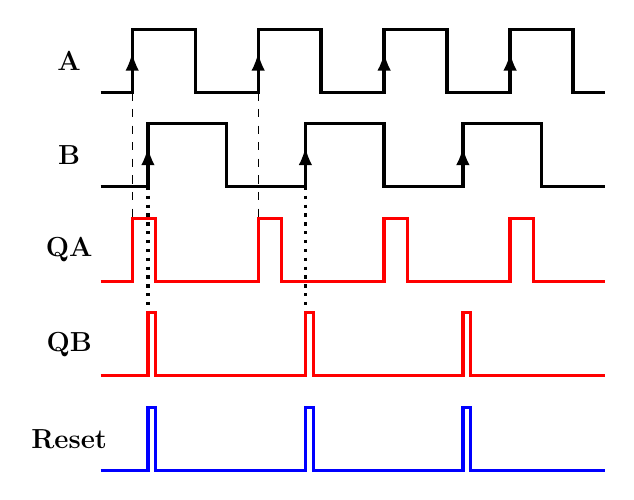
\begin{tikzpicture}[scale=0.4, transform shape]
            \draw[very thick](1+0,4)--++(1,0)--++(0,2)--++(2,0)--++(0,-2)--++(2,0)
                                   --++(0,2)--++(2,0)--++(0,-2)--++(2,0)
                                   --++(0,2)--++(2,0)--++(0,-2)--++(2,0)
                                   --++(0,2)--++(2,0)--++(0,-2)--++(1,0);
            \draw[very thick](1,1)--++(1,0)--++(0.5,0)--++(0,2)--++(2.5,0)--++(0,-2)--++(2.5,0)
                                   --++(0,2)--++(2.5,0)--++(0,-2)--++(2.5,0)
                                   --++(0,2)--++(2.5,0)--++(0,-2)--++(2.5-0.5,0);
        %tratteggi
        \draw[dashed](2,4)--++(0,-4);
        \draw[dashed](6,4)--++(0,-4);
        \draw[dotted,very thick](2.5,1)--++(0,-4);
        \draw[dotted,very thick](7.5,1)--++(0,-4);
        %output A
            \draw[very thick,red](1+0,-2)--++(1,0)--++(0,2)--++(0.5+0.25,0)--++(0,-2)--++(2-0.5-0.25,0)
                                   --++(2,0)--++(0,2)--++(0.5+0.25,0)--++(0,-2)--++(2-0.5-0.25,0)
                                   --++(2,0)--++(0,2)--++(0.5+0.25,0)--++(0,-2)--++(2-0.5-0.25,0)
                                   --++(2,0)--++(0,2)--++(0.5+0.25,0)--++(0,-2)--++(2+1-0.5-0.25,0);
        %output B
            \draw[very thick,red](1,-5)--++(1,0)--++(0.5,0)--++(0,2)--++(0.25,0)--++(0,-2)--++(2+1-0.25,0)
                                   --++(2,0)--++(0,2)--++(0.25,0)--++(0,-2)--++(2+1-0.25,0)
                                   --++(2,0)--++(0,2)--++(0.25,0)--++(0,-2)--++(2+1+1+0.25,0);
        %reset:
            \draw[very thick,blue](1,-8)--++(1,0)--++(0.5,0)--++(0,2)--++(0.25,0)--++(0,-2)--++(2+1-0.25,0)
                                    --++(2,0)--++(0,2)--++(0.25,0)--++(0,-2)--++(2+1-0.25,0)
                                    --++(2,0)--++(0,2)--++(0.25,0)--++(0,-2)--++(2+1+1+0.25,0);
        %label
        \node at (0,5)[]{\Huge \textbf{A}};
        \node at (0,2)[]{\Huge \textbf{B}};
        \node at (0,-1)[]{\Huge \textbf{QA}};
        \node at (0,-4)[]{\Huge \textbf{QB}};
        \node at (0,-7)[]{\Huge \textbf{Reset}};

        %clk A
        \draw[-latex,very thick](2,5)--++(0,0.25);
        \draw[-latex,very thick](6,5)--++(0,0.25);
        \draw[-latex,very thick](10,5)--++(0,0.25);
        \draw[-latex,very thick](14,5)--++(0,0.25);
        %clk B
        \draw[-latex,very thick](2.5,2)--++(0,0.25);
        \draw[-latex,very thick](7.5,2)--++(0,0.25);
        \draw[-latex,very thick](12.5,2)--++(0,0.25);

        \end{tikzpicture}
        \caption{Caption for image 1}
        \label{fig:image1}
    \end{minipage}%
    \hfill
    \begin{minipage}{0.45\textwidth}
        \centering
        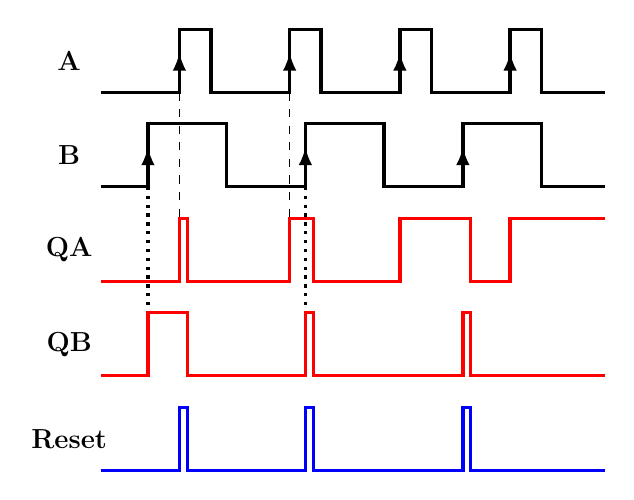
\begin{tikzpicture}[scale=.4, transform shape]
            \draw[very thick](1+0,4)--++(2.5,0)--++(0,2)--++(1,0)--++(0,-2)--++(2.5,0)
                                   --++(0,2)--++(1,0)--++(0,-2)--++(2.5,0)
                                   --++(0,2)--++(1,0)--++(0,-2)--++(2.5,0)
                                   --++(0,2)--++(1,0)--++(0,-2)--++(2,0);
            \draw[very thick](1,1)--++(1,0)--++(0.5,0)--++(0,2)--++(2.5,0)--++(0,-2)--++(2.5,0)
                                   --++(0,2)--++(2.5,0)--++(0,-2)--++(2.5,0)
                                   --++(0,2)--++(2.5,0)--++(0,-2)--++(2.5-0.5,0);
        %tratteggi
        \draw[dashed](3.5,4)--++(0,-4);
        \draw[dashed](7,4)--++(0,-4);
        \draw[dotted,very thick](2.5,1)--++(0,-4);
        \draw[dotted,very thick](7.5,1)--++(0,-4);
        %output A
            \draw[very thick,red](1+0,-2)--++(2.5,0)--++(0,2)--++(0.25,0)--++(0,-2)--++(2-1-0.25,0)
                                   --++(2.5,0)--++(0,2)--++(0.25+0.5,0)--++(0,-2)--++(2-1-0.5-0.25,0)
                                   --++(2.5,0)--++(0,2)--++(2+0.25,0)--++(0,-2)--++(2-1-0.5-0.25,0)
                                   --++(1,0)--++(0,2)--++(0.25,0)--++(2+1.5-0.5-0.25,0);
        %output B
        \draw[very thick,red](1+0,-5)--++(1.5,0)--++(0,2)--++(1+0.25,0)--++(0,-2)--++(2-0.25,0)
                                --++(2,0)--++(0,2)--++(0.25,0)--++(0,-2)--++(2+1.5-0.5-0.25,0)
                                --++(2,0)--++(0,2)--++(0.25,0)--++(0,-2)--++(2+3-0.5-0.25,0);
        %reset:
            \draw[very thick,blue](1,-8)--++(1,0)--++(1.5,0)--++(0,2)--++(0.25,0)--++(0,-2)--++(2-0.25,0)
                                    --++(2,0)--++(0,2)--++(0.25,0)--++(0,-2)--++(2+1-0.25,0)
                                    --++(2,0)--++(0,2)--++(0.25,0)--++(0,-2)--++(2+1+1+0.25,0);
        %label
        \node at (0,5)[]{\Huge \textbf{A}};
        \node at (0,2)[]{\Huge \textbf{B}};
        \node at (0,-1)[]{\Huge \textbf{QA}};
        \node at (0,-4)[]{\Huge \textbf{QB}};
        \node at (0,-7)[]{\Huge \textbf{Reset}};

         %clk A
         \draw[-latex,very thick](3.5,5)--++(0,0.25);
         \draw[-latex,very thick](7,5)--++(0,0.25);
         \draw[-latex,very thick](10.5,5)--++(0,0.25);
         \draw[-latex,very thick](14,5)--++(0,0.25);
         %clk B
         \draw[-latex,very thick](2.5,2)--++(0,0.25);
         \draw[-latex,very thick](7.5,2)--++(0,0.25);
         \draw[-latex,very thick](12.5,2)--++(0,0.25);

        \end{tikzpicture}
        \caption{Caption for image 2}
        \label{fig:image2}
    \end{minipage}
    \caption{Overall caption for the figure}
    \label{fig:two_images}
\end{figure}
\subsection{Charge pump}
\begin{figure}
    \begin{circuitikz}
        \ctikzset{
    bipoles/capacitor/height=0.4,
    bipoles/capacitor/width=0.2 
}
        \draw (0,0)node[vcc]{Vcc} to[isource, l=$I_{cp}$]++(0,-2) 
        to [nos,mirror,invert] ++(0,-1)
        --++(0,-0.25)coordinate(out)--++(0,-0.25)
        to [nos,mirror,invert] ++(0,-1)
        to[isource, l=$I_{cp}$]++(0,-2) node[ground]{};
        %out
        \draw (out)--++(1.5,0)
        to[C]++(0,-1.25)node[tlground]{};
        %frecce
        \draw[-latex](-1.25,-4)node[left]{QB}--++(1,0);
        \draw[-latex](-1.25,-2.5)node[left]{QA}--++(1,0);

        % charge, discharge
        \draw[-latex,blue](0.25,-1.5)..controls (0.25,-3) and (0.75,-3)..(1.25,-3)node[above]{\small charge};
        \begin{scope}[shift={(0,-6.5)},yscale=-1]
            \draw[latex-,red](0.25,-1.5)node[right]{\small discharge}..controls (0.25,-3) and (0.75,-3)..(1.25,-3);
        \end{scope}

        %label on, off
        \draw[red](-1.85,-4)node[left]{ON,};
        \draw[red](-1.85,-2.5)node[left]{OFF,};
        \draw[blue](-2.75,-4)node[left]{ON,};
        \draw[blue](-2.75,-2.5)node[left]{OFF,};

    \end{circuitikz}
\end{figure}

\begin{figure}
    \begin{tikzpicture}
        \draw[red,thick] (0,0)--++(0,2)--++(1,0)--++(0,-2)--++(2,0)
        --++(0,2)--++(1,0)--++(0,-2)--++(2,0)
        --++(0,2)--++(1,0)--++(0,-2)--++(2,0)
        --++(0,2)--++(1,0)--++(0,-2)--++(2,0);
        \draw[blue,thick] (0,-6)--++(1,1)--++(2,0)
        --++(1,1)--++(2,0)
        --++(1,1)--++(2,0)
        --++(1,1)--++(2,0);
        %tratteggi
        \draw[dashed](0,0)--++(0,-6);
        \draw[dashed](1,0)--++(0,-5);
        \draw[dashed](3,0)--++(0,-5);
        \draw[dashed](4,0)--++(0,-4);
        \draw[dashed](6,0)--++(0,-4);
        \draw[dashed](7,0)--++(0,-3);
        \draw[dashed](9,0)--++(0,-3);
        \draw[dashed](10,0)--++(0,-2);
                
    \end{tikzpicture}
\end{figure}
\subsection{PFDCP behvioral simulation}
\subsection{Charge pump PLL}
\subsubsection{Stability considerations}
\subsection{Open loop bandwidth and phase margin}
\subsection{high order pll}
\begin{figure}
    \begin{circuitikz}
        \ctikzset{
    bipoles/capacitor/height=0.4,bipoles/capacitor/width=0.2,
    bipoles/resistor/height=0.3,bipoles/resistor/width=0.4 
}
        \draw (0,0)node[vcc]{Vcc} to[isource, l=$I_{cp}$]++(0,-2) 
        to [nos,mirror,invert] ++(0,-1)
        --++(0,-0.25)coordinate(out)--++(0,-0.25)
        to [nos,mirror,invert] ++(0,-1)
        to[isource, l=$I_{cp}$]++(0,-2) node[ground]{};
        %out
        \draw (out)--++(3,0)
        to[C]++(0,-1.25)node[tlground]{};
        \draw (out)--++(1.5,0)
        to[R]++(0,-1.25)
        to[C]++(0,-1.25)node[tlground]{};
        %frecce
        \draw[-latex](-1.25,-4)node[left]{QB}--++(1,0);
        \draw[-latex](-1.25,-2.5)node[left]{QA}--++(1,0);
    \end{circuitikz}
\end{figure}

\begin{figure}
    \begin{tikzpicture}
    %asse x
    \draw[-latex,thick] (0,0)--++(7,0);
    %asse y
    \draw[-latex,thick] (0,0)--++(0,6);
    %grafico
    \draw[blue,very thick](0.25,5)--(2,3)--(4,2)--(6,-0.05);

    \begin{scope}[shift={(0,2)}]
        %asse x
        \draw[-latex,thick](0,-4)--++(7,0);
        %asse y
        \draw[-latex,thick](0,-9)--++(0,6);
        %gradi
        \node at (0,-8)[left]{-180};
        \node at (0,-7)[left]{-135};
        \node at (0,-6)[left]{-90};
        %grafico
        \draw[red, very thick](0,-8)..controls (3.5,-8) and (1,-4).. (7,-7);
    \end{scope}

    %tratteggi
    \draw[dashed](2,3)--++(0,-8);
    \draw[dashed](4,2)--++(0,-5.9);
    \draw[dashed](0,-5)--++(2,0);

    \end{tikzpicture}
\end{figure}